\section{Prototyping}
\label{sec:prototype}

In this paper, we provide a prototyping of ICT platforms for mobility
CPS applications, particularly taking an example of autonomous driving.
We apply the cloud computing paradigm for autonomous driving to
complement wimpy vehicular embedded systems.
One of the major goals of this cloud-based autonomous driving system is
to offload the computational requirement of autonomic control and
environmental perception to remote HPC servers from local vehicular
systems.
We focus on ICT platforms.
Hence, the implementations of autonomic control and environmental
perception for autonomous driving are outside the scope of this paper.
Interested readers are encouraged to refer to our different
contributions \cite{Hirabayashi13, Kagami13}.

In the rest of this section, we present two ICT platforms for the
development of cloud-based autonomous driving.
The first platform is a smartphone application that controls the vehicle
from remote sources.
The second platform is also a smartphone application that transfers
captured images to the HPC server as fast as possible.

\subsection{Remote Vehicle Control}

\begin{figure}[!t]
 \centering
 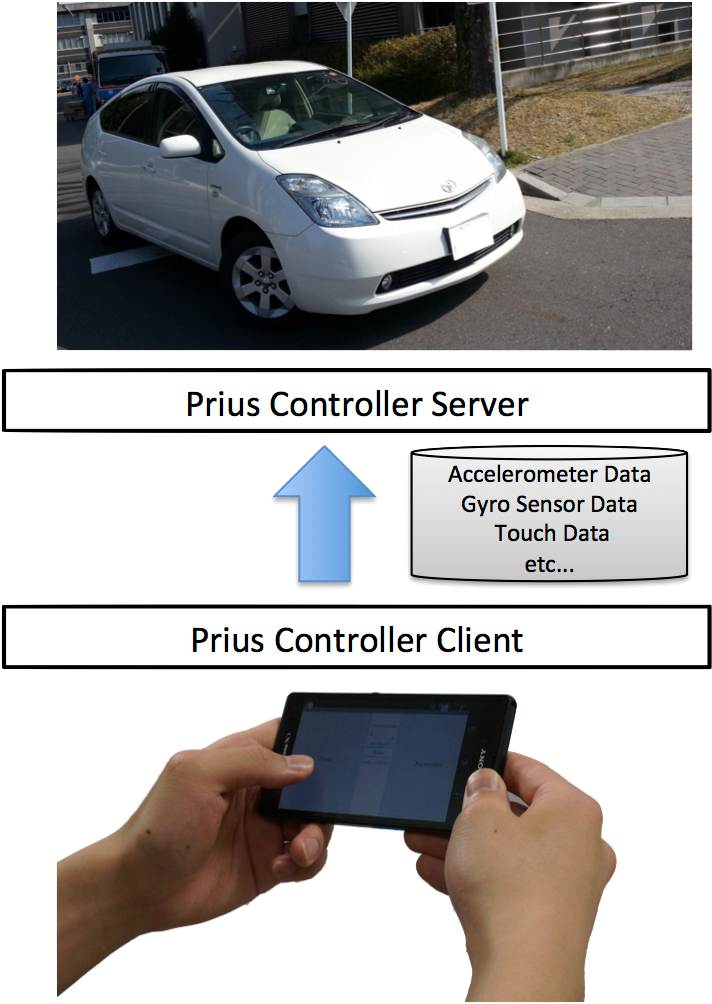
\includegraphics[width=0.6\hsize]{fig/Andrive.pdf}
 \caption{A smartphone application for remote vehicle control.}
 \label{fig:andrive}
\end{figure}

We have a TOYOTA Prius that is modified to be able to overwrite the
control of steering, accel, and break from the computer.
This computer called ``local master computer'' is connected to an
supplemental embedded device board that can directly send signals to the
internale wire system controlling the vehicle.
We omit a detailed description of this autonomous driving system, as our
primary focus is the quantification of overhead.

Fig. \ref{fig:andrive} shows a conceptual architecture of our
experimental remote vehicle control system.
We make use of a commodity smartphone to send the control command to the
local master computer equipped within the vehicle through the network.
The smartphone application determines the steering angle from the gyro
sensor while the accel and the break strokes are controlled by the
graphics user interface.
Thus, we can intuitively use a smartphone as if it were a game
controller of the vehicle remotely.

\subsection{Networked Image Processing}

\begin{figure}[!t]
 \centering
 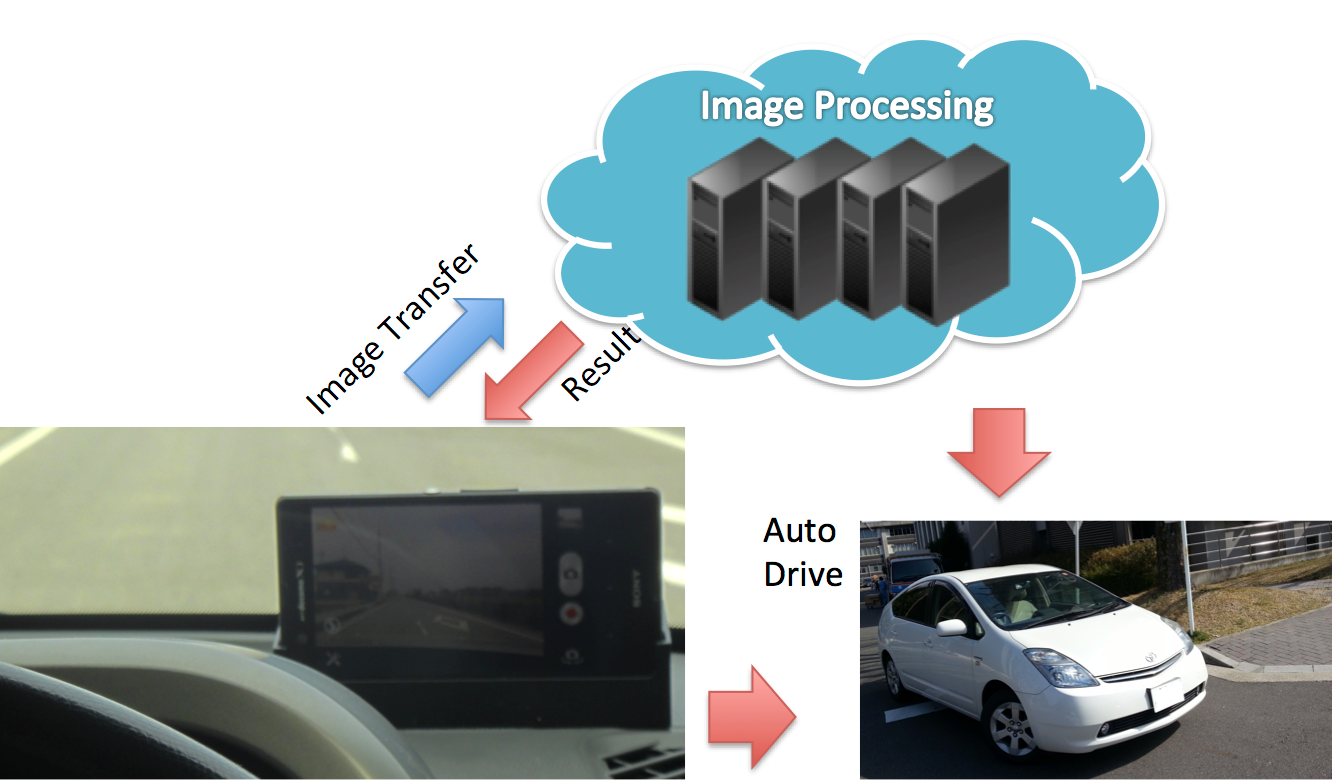
\includegraphics[width=0.9\hsize]{fig/TIPIC.pdf}
 \caption{Networked image processing.}
 \label{fig:tipic}
\end{figure}

Environmental perception is composed of compute-intensive tasks.
Perception algorithms are often complex and the volume of input data
from laser sensors and high-resolution cameras is not afforable for
mobile embedded systems.
Therefore it is significant if we can offload these compute-intensive
tasks to the cloud in real-time.

Fig. \ref{fig:tipic} shows a conceptual architecture of our experimental
networked image processing system.
We capture images in real-time from commodity smartphones attached in
the vehicle and transfer them over the network to the HPC server where
the actual image processing tasks are executing.
The results of image processing such as the detected vehicles and
pedestrians are fed back to the vehicular embedded system.
Although we have implemented several variants of state-of-the-art image
processing algorithms \cite{Hirabayashi13}, we exclude them from the
scope of this paper.
Alternatively we investigate if commodity ICT platforms can meet the
requirement of throughput and latency for image transfers.

\begin{figure}[!t]
 \centering
 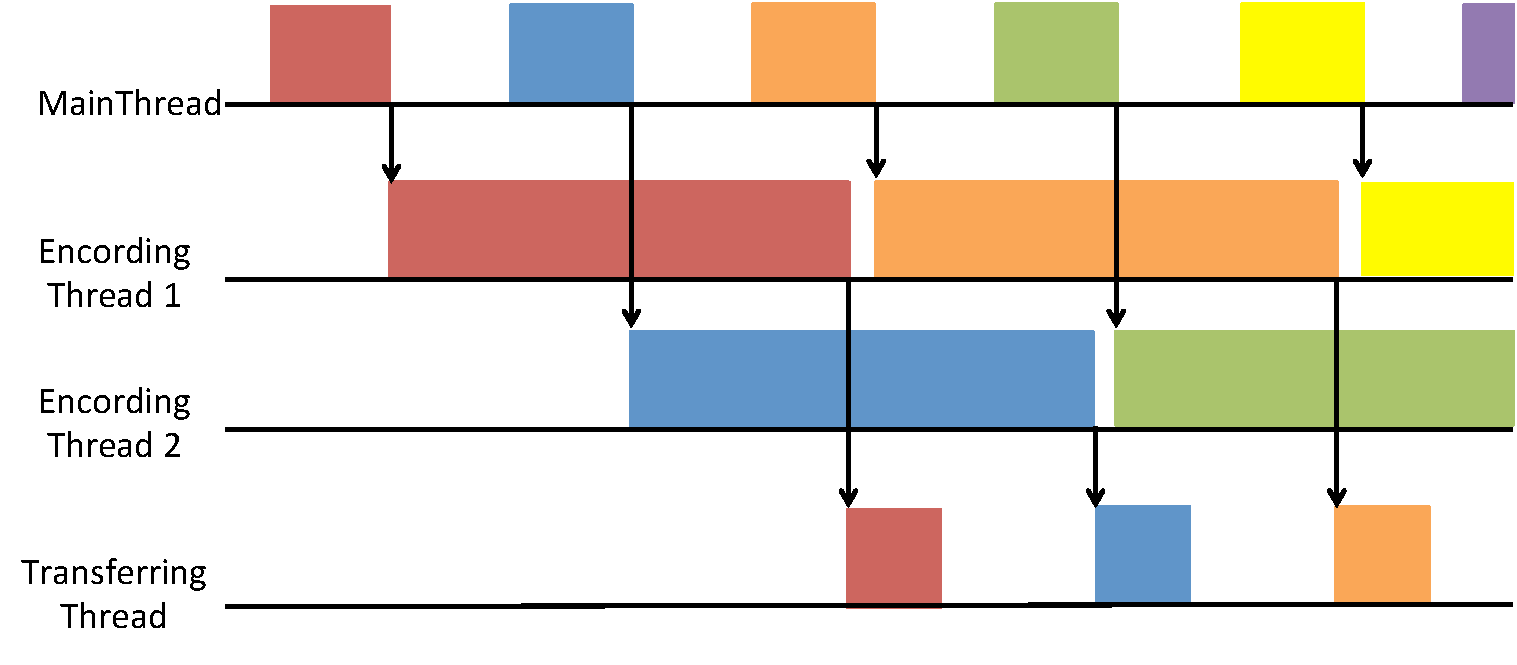
\includegraphics[width=0.9\hsize]{fig/multithread.pdf}
 \caption{Multithreading of image transfers.}
 \label{fig:multithread}
\end{figure}

Unlike control commands, the size of an image is large and it generates
additional latency for the transfer.
For example, each image transfer is composed of (i) capturing an image,
(ii) encoding that image, and (iii) transferring the encoded image.
Since these three stages can be pipelined, the total throughput would
benefit from multithreading and a multicore processor.
Furthermore, we have observed that the encoding stage is much longer
than the capture and the transfer stages when we use a smartphone as a
client due to its wimpy embedded processor performance.
This means that the effective rate of image capture and transfer may be
limitted to the execution time of encodling.
In order to maximize the image transfer throughput on an embedded
multicore processor, we increase the number of threads for encoding as
shown in Fig. \ref{fig:multithread}.
In this example, one can see that the second (blue) transfer does not
have to stall before the encoding stage because another thread is
available for encoding whereas it would stall due to the preceding
encoding process if there is only one thread available for encoding.
Thus, we suggest that networked image processing using smartphones
should make use of the multithreading capability and the parallelism of
embedded multicore processors.